
To detect circles in the image, we used the well-known technique Hough Circle Transform.

To simplify the image in which we had to search for circles, we first applied a processing based on local variance.
Given an image $I(x,y)$, firstly the local mean $\mu(x,y)$ is computed on a kernel of size $15 \times 15$ centered in $(x,y)$ as follows:
\begin{equation}
    \mu(x,y) = \frac{1}{|K|} \sum_{(u,v) \in K} I(x+u,y+v)\ ,
\end{equation}
similarly, the local mean of the squared intensity values:
\begin{equation}
    \mu_2(x,y) = \frac{1}{|K|} \sum_{(u,v) \in K} I^2(x+u,y+v)\ .
\end{equation}
The local variance is then defined as:
\begin{equation}
    \sigma^2(x,y) = \mu_2(x,y) - \mu^2(x,y)\ .
\end{equation}
After normalizing to the interval $[0,255]$, we applied a threshold to obtain a binary mask that highlights strong local variance values:
\begin{equation}
    M(x,y) = \begin{cases}
        1 & \text{if } \sigma^2(x,y) > 30 \\[5pt]
        0 & \text{otherwise}
    \end{cases}\ .
\end{equation}
This technique has a similar effect to edge detection, but it is more robust to noise and illumination changes.
In fact, it brought several advantages:
\begin{itemize}
    \item it almost ignores internal texture of the coins, which is not useful for circle detection but it will be relevant for the classification step using template matching;
    \item it enhances the external edges of the coins, making the detection easier and more precise;
    \item it is also able to remove hands from the detection, since they have a low local variance as they are uniform.
\end{itemize}

\begin{figure}[H]
    \centering
    \subfloat[Local variance computation result. \label{Detection:fig:local_variance}]{
        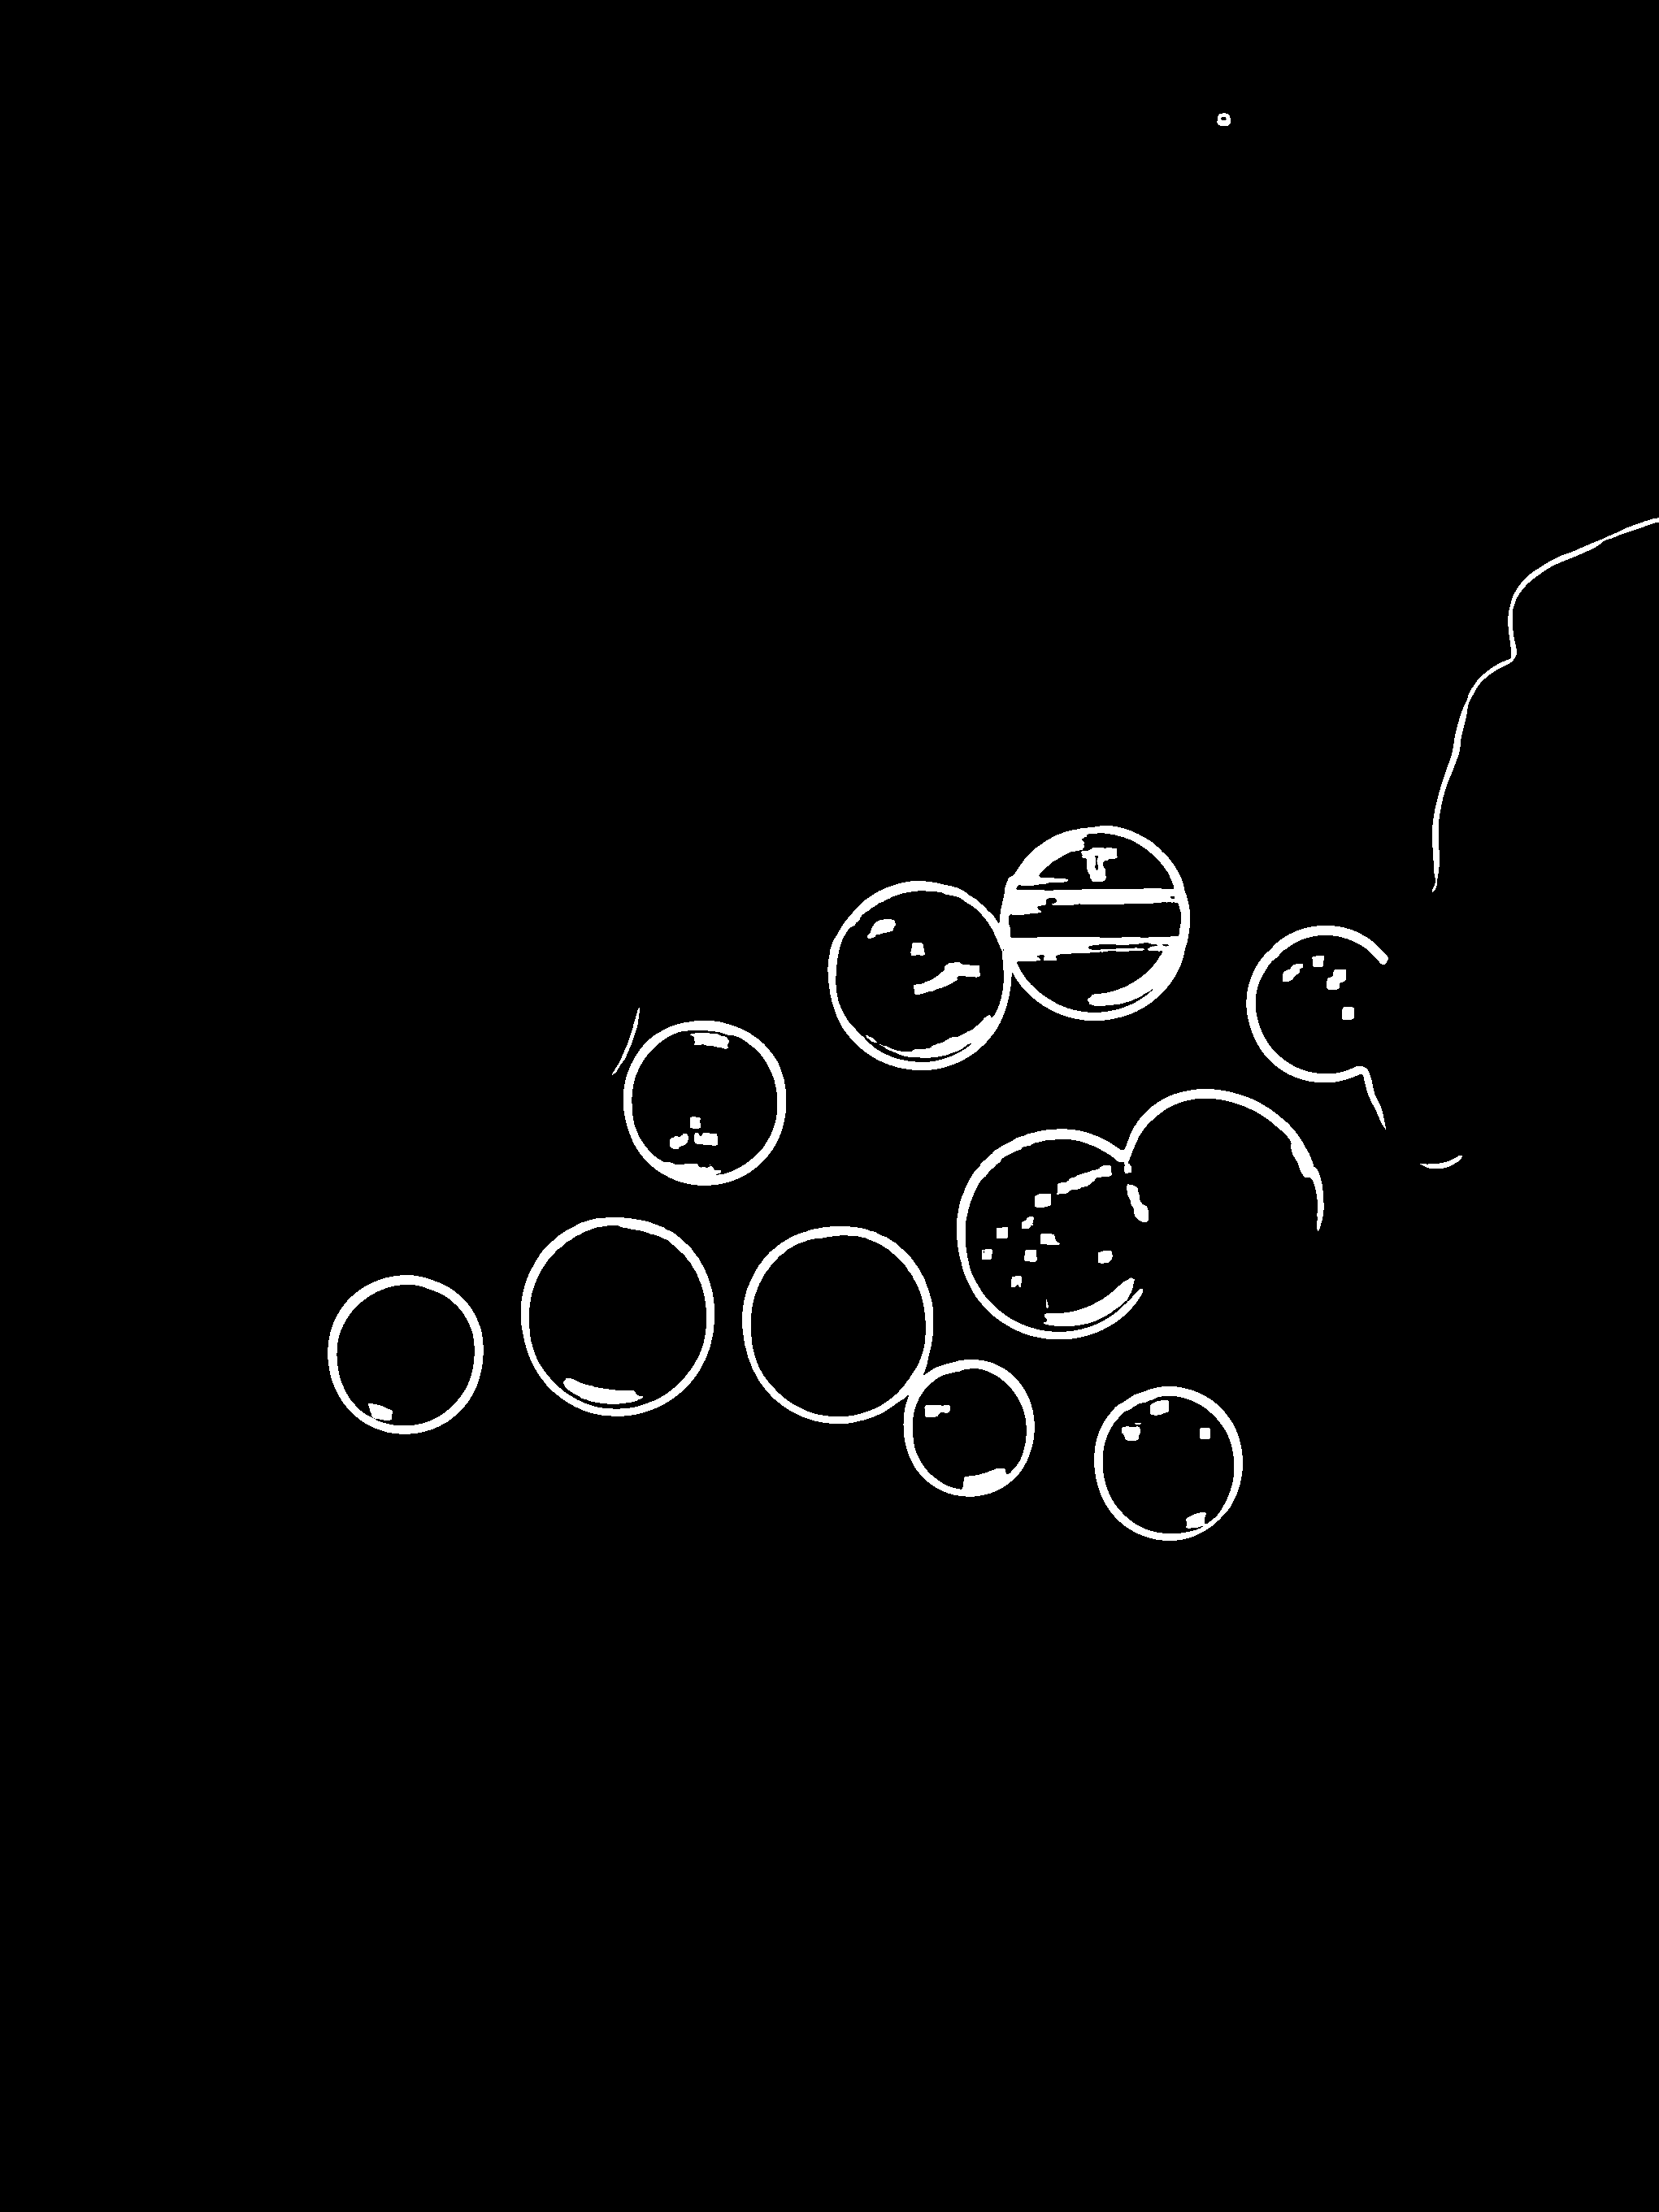
\includegraphics[width=0.35\textwidth]{Immagini/local_variance.png}
    }\hspace{1cm}
    \subfloat[Hough circles transform on a. \label{Detection:fig:detected_circles}]{
        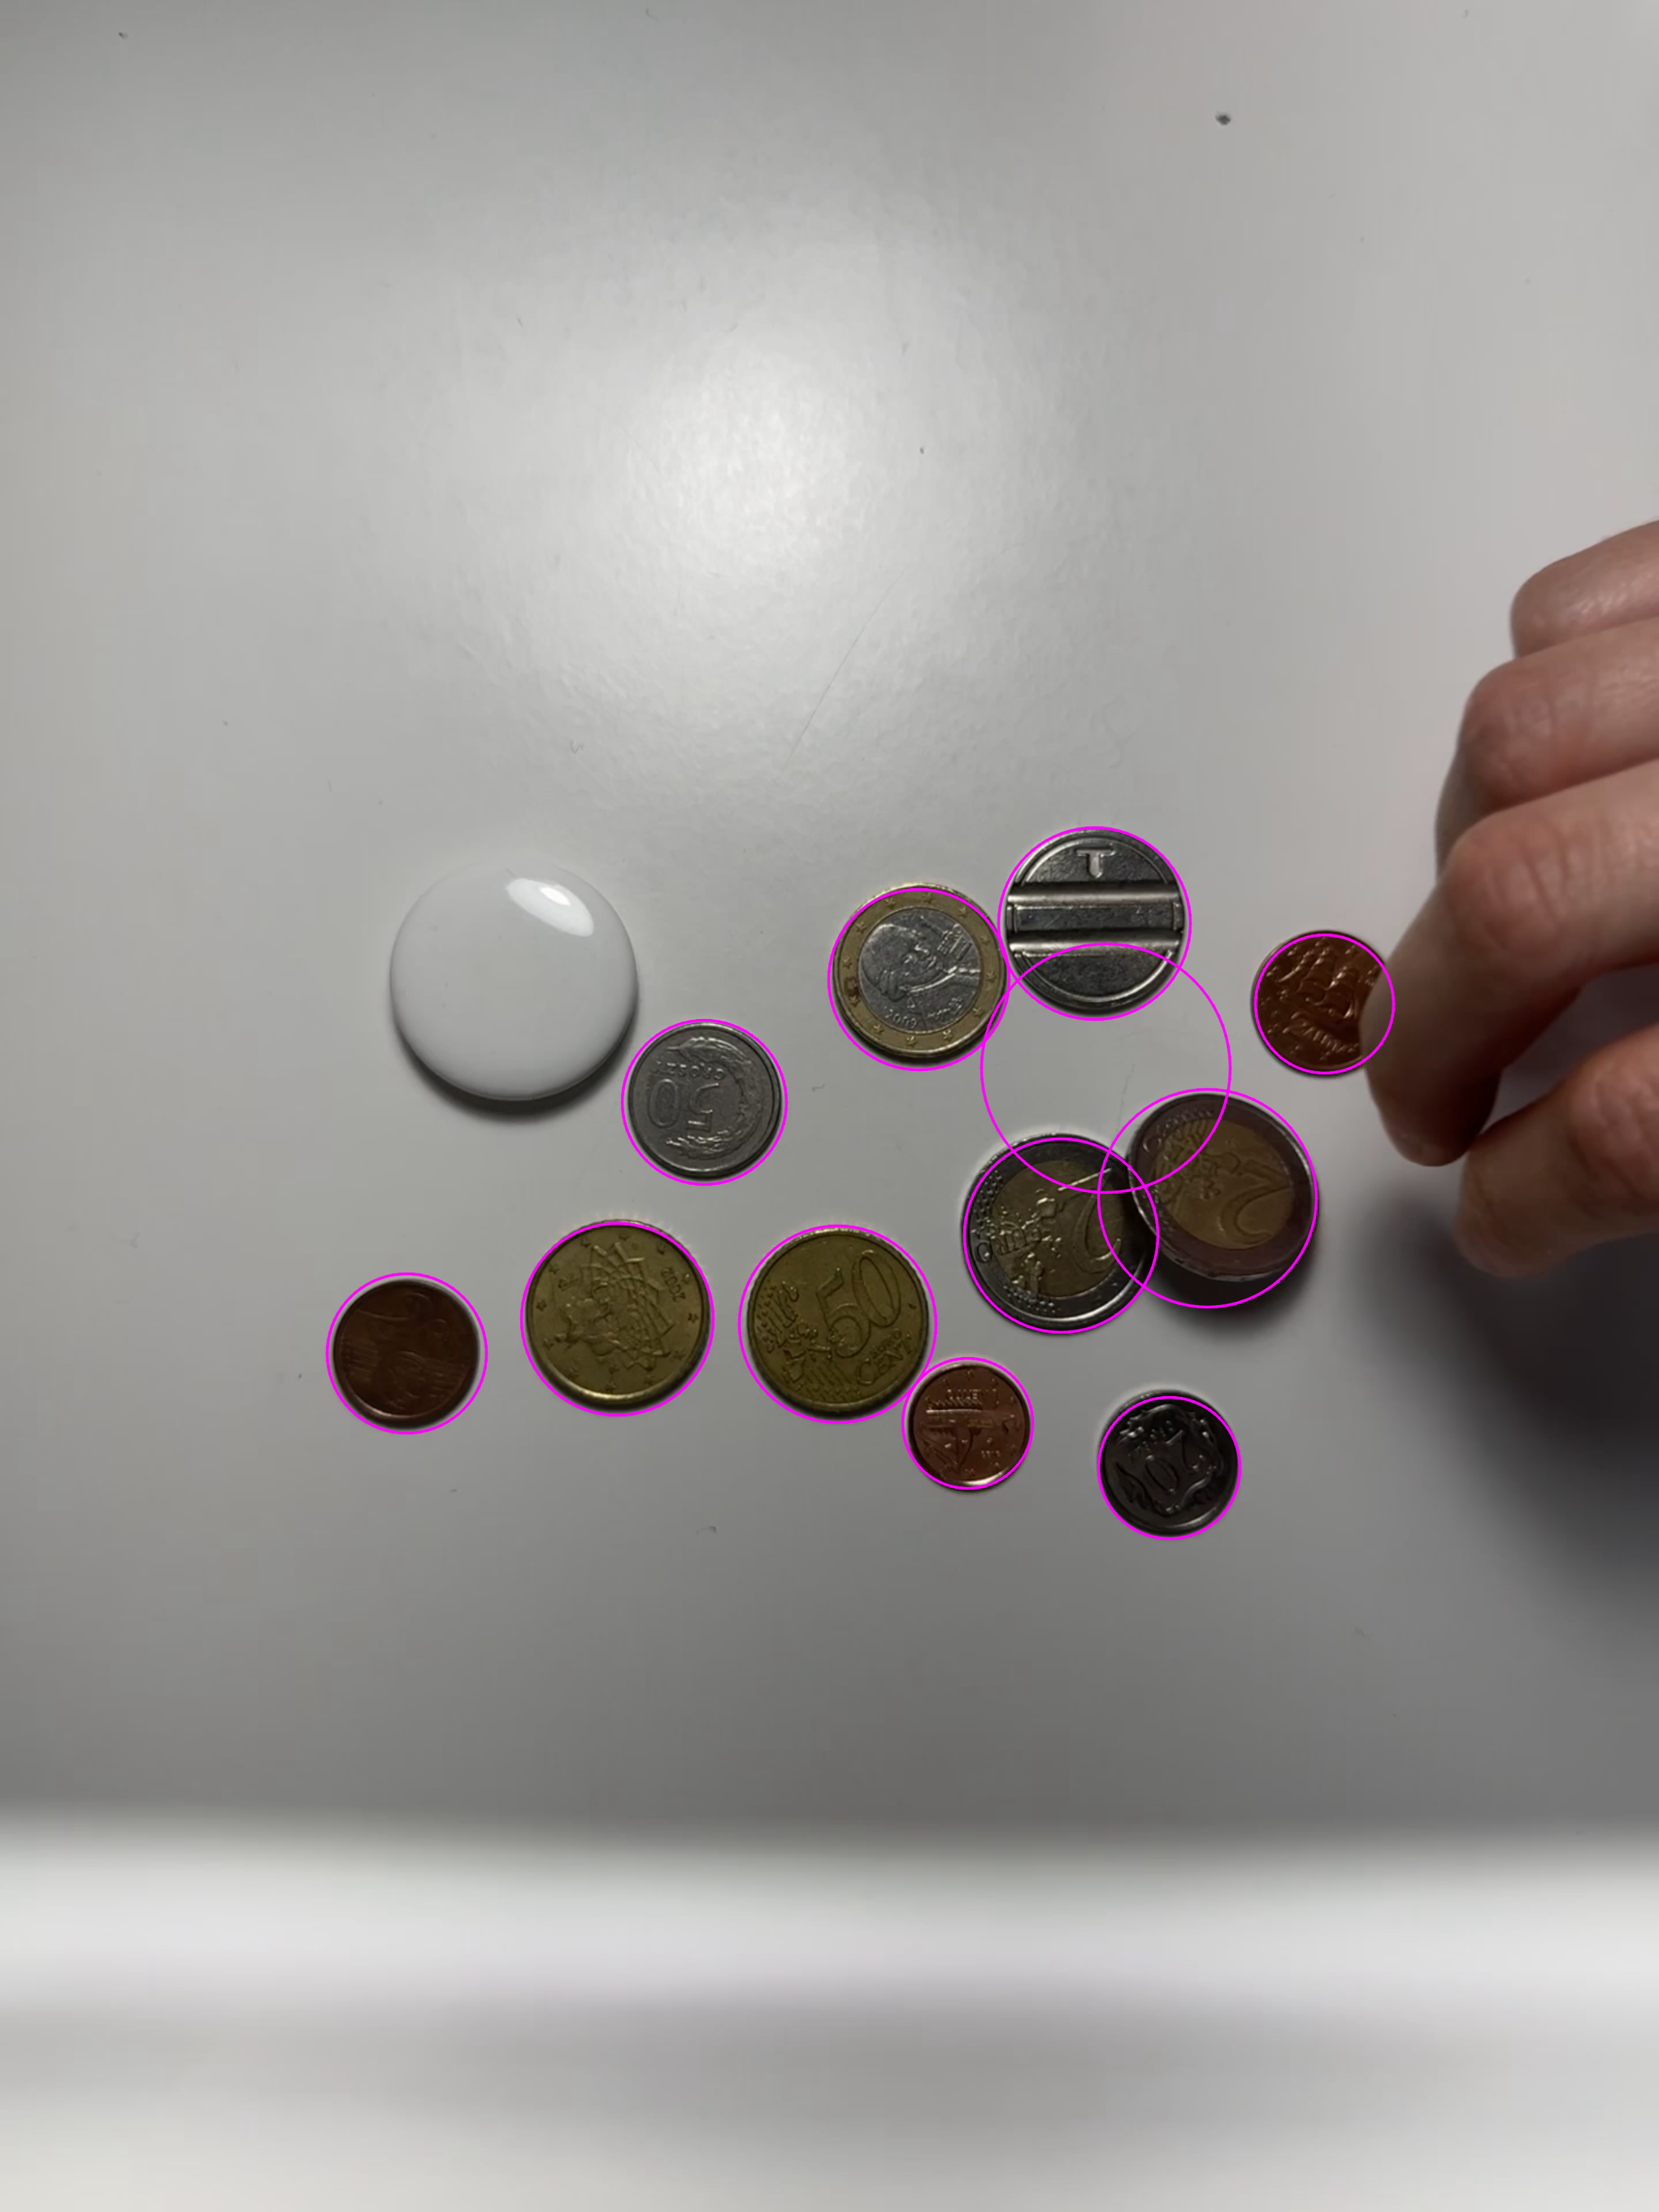
\includegraphics[width=0.35\textwidth]{Immagini/detected_circles.png}
    }
    \caption{Hough circles result after applying local variance processing.}
    \label{Detection:fig:circle_detection_intermediate}
\end{figure}

After this preprocessing, we applied the Hough Circle Transform to detect circles in the image (Figure~\ref{Detection:fig:circle_detection_intermediate}).

To further improve the detection, we exploited the color information of the coins.
In fact, euro coins contain only three colors: gold, silver and copper.
Actually there is no completely silver coin, since the 1 and 2 euro coins contain also gold.
So we decided to compute a mask containing only the gold and copper colors, which are the most distinguishable ones and are not usually present in any other objects.
To do this, we converted the image to the LAB color space and created a mask by thresholding the \textbf{a} and \textbf{b} channels.
This way, we were able to filter out all the circles that did not contain enough gold or copper color inside them independently from the lightness (Figure~\ref{Detection:fig:circle_detection_final}).

\begin{figure}[H]
    \centering
    \subfloat[Gold or copper thresholding mask. \label{Detection:fig:gold_or_copper}]{
        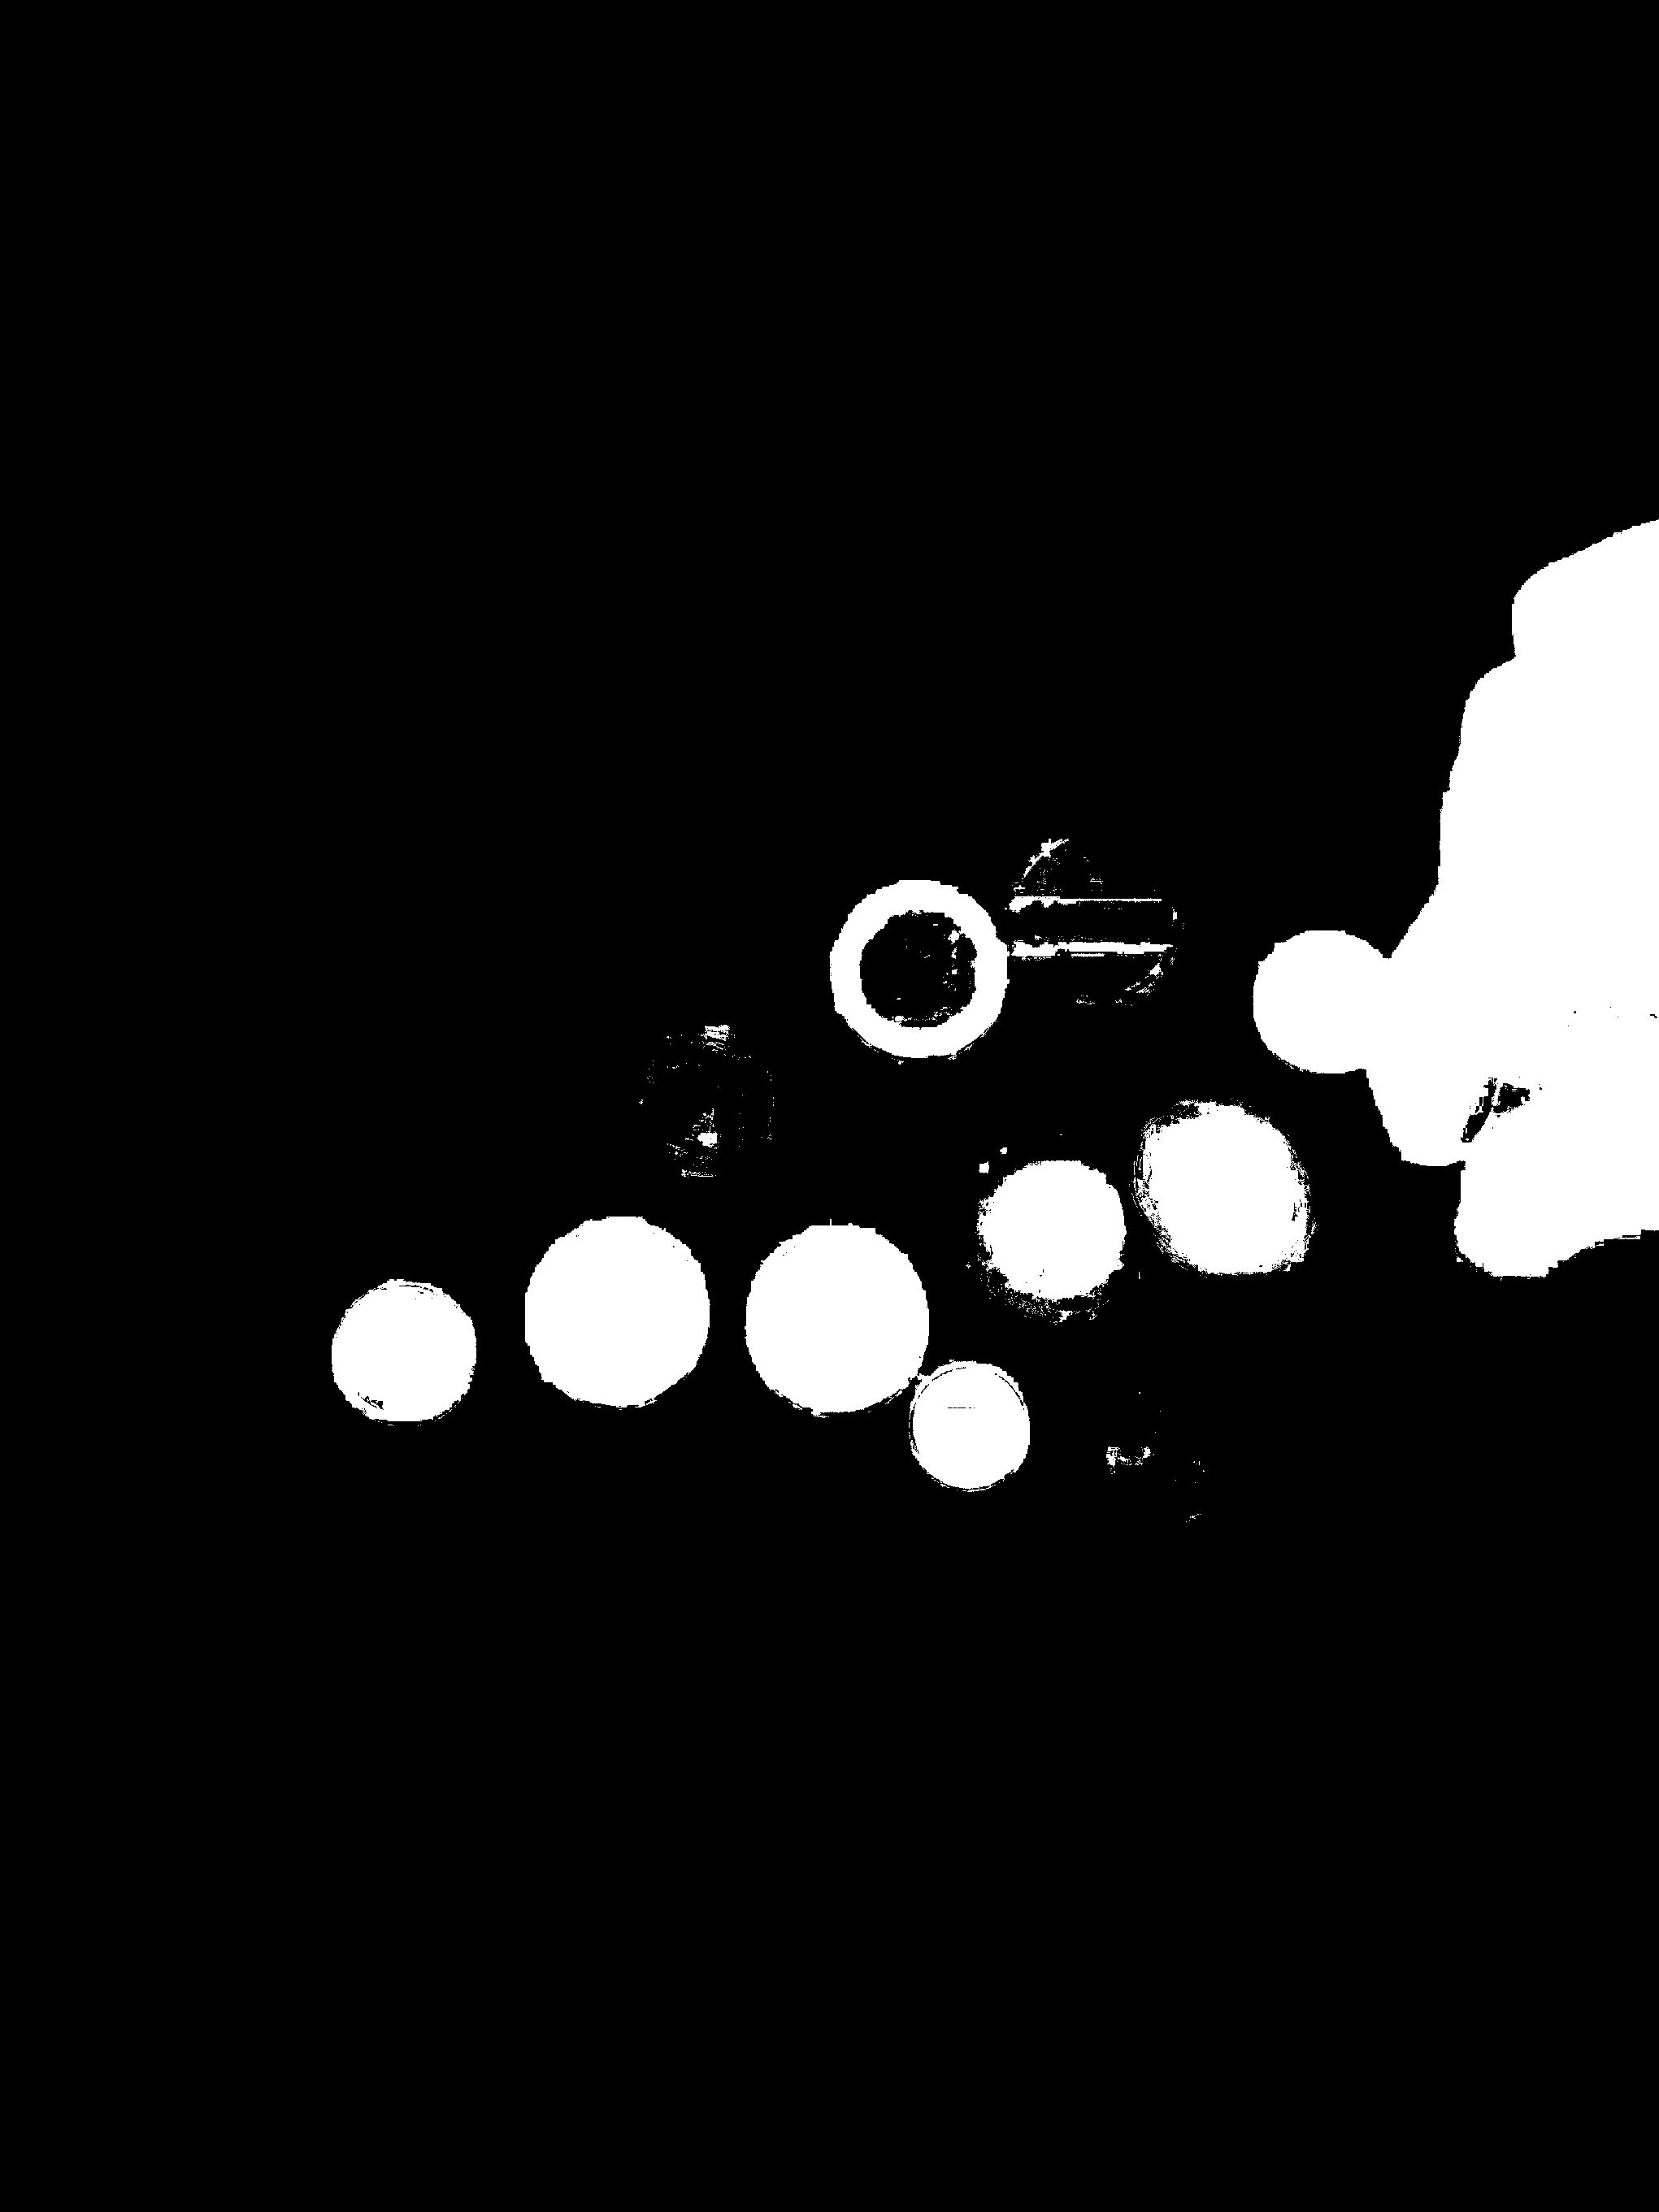
\includegraphics[width=0.35\textwidth]{Immagini/gold_or_copper.png}
    }\hspace{1cm}
    \subfloat[Filtered circles using the mask a. \label{Detection:fig:remaining_circles}]{
        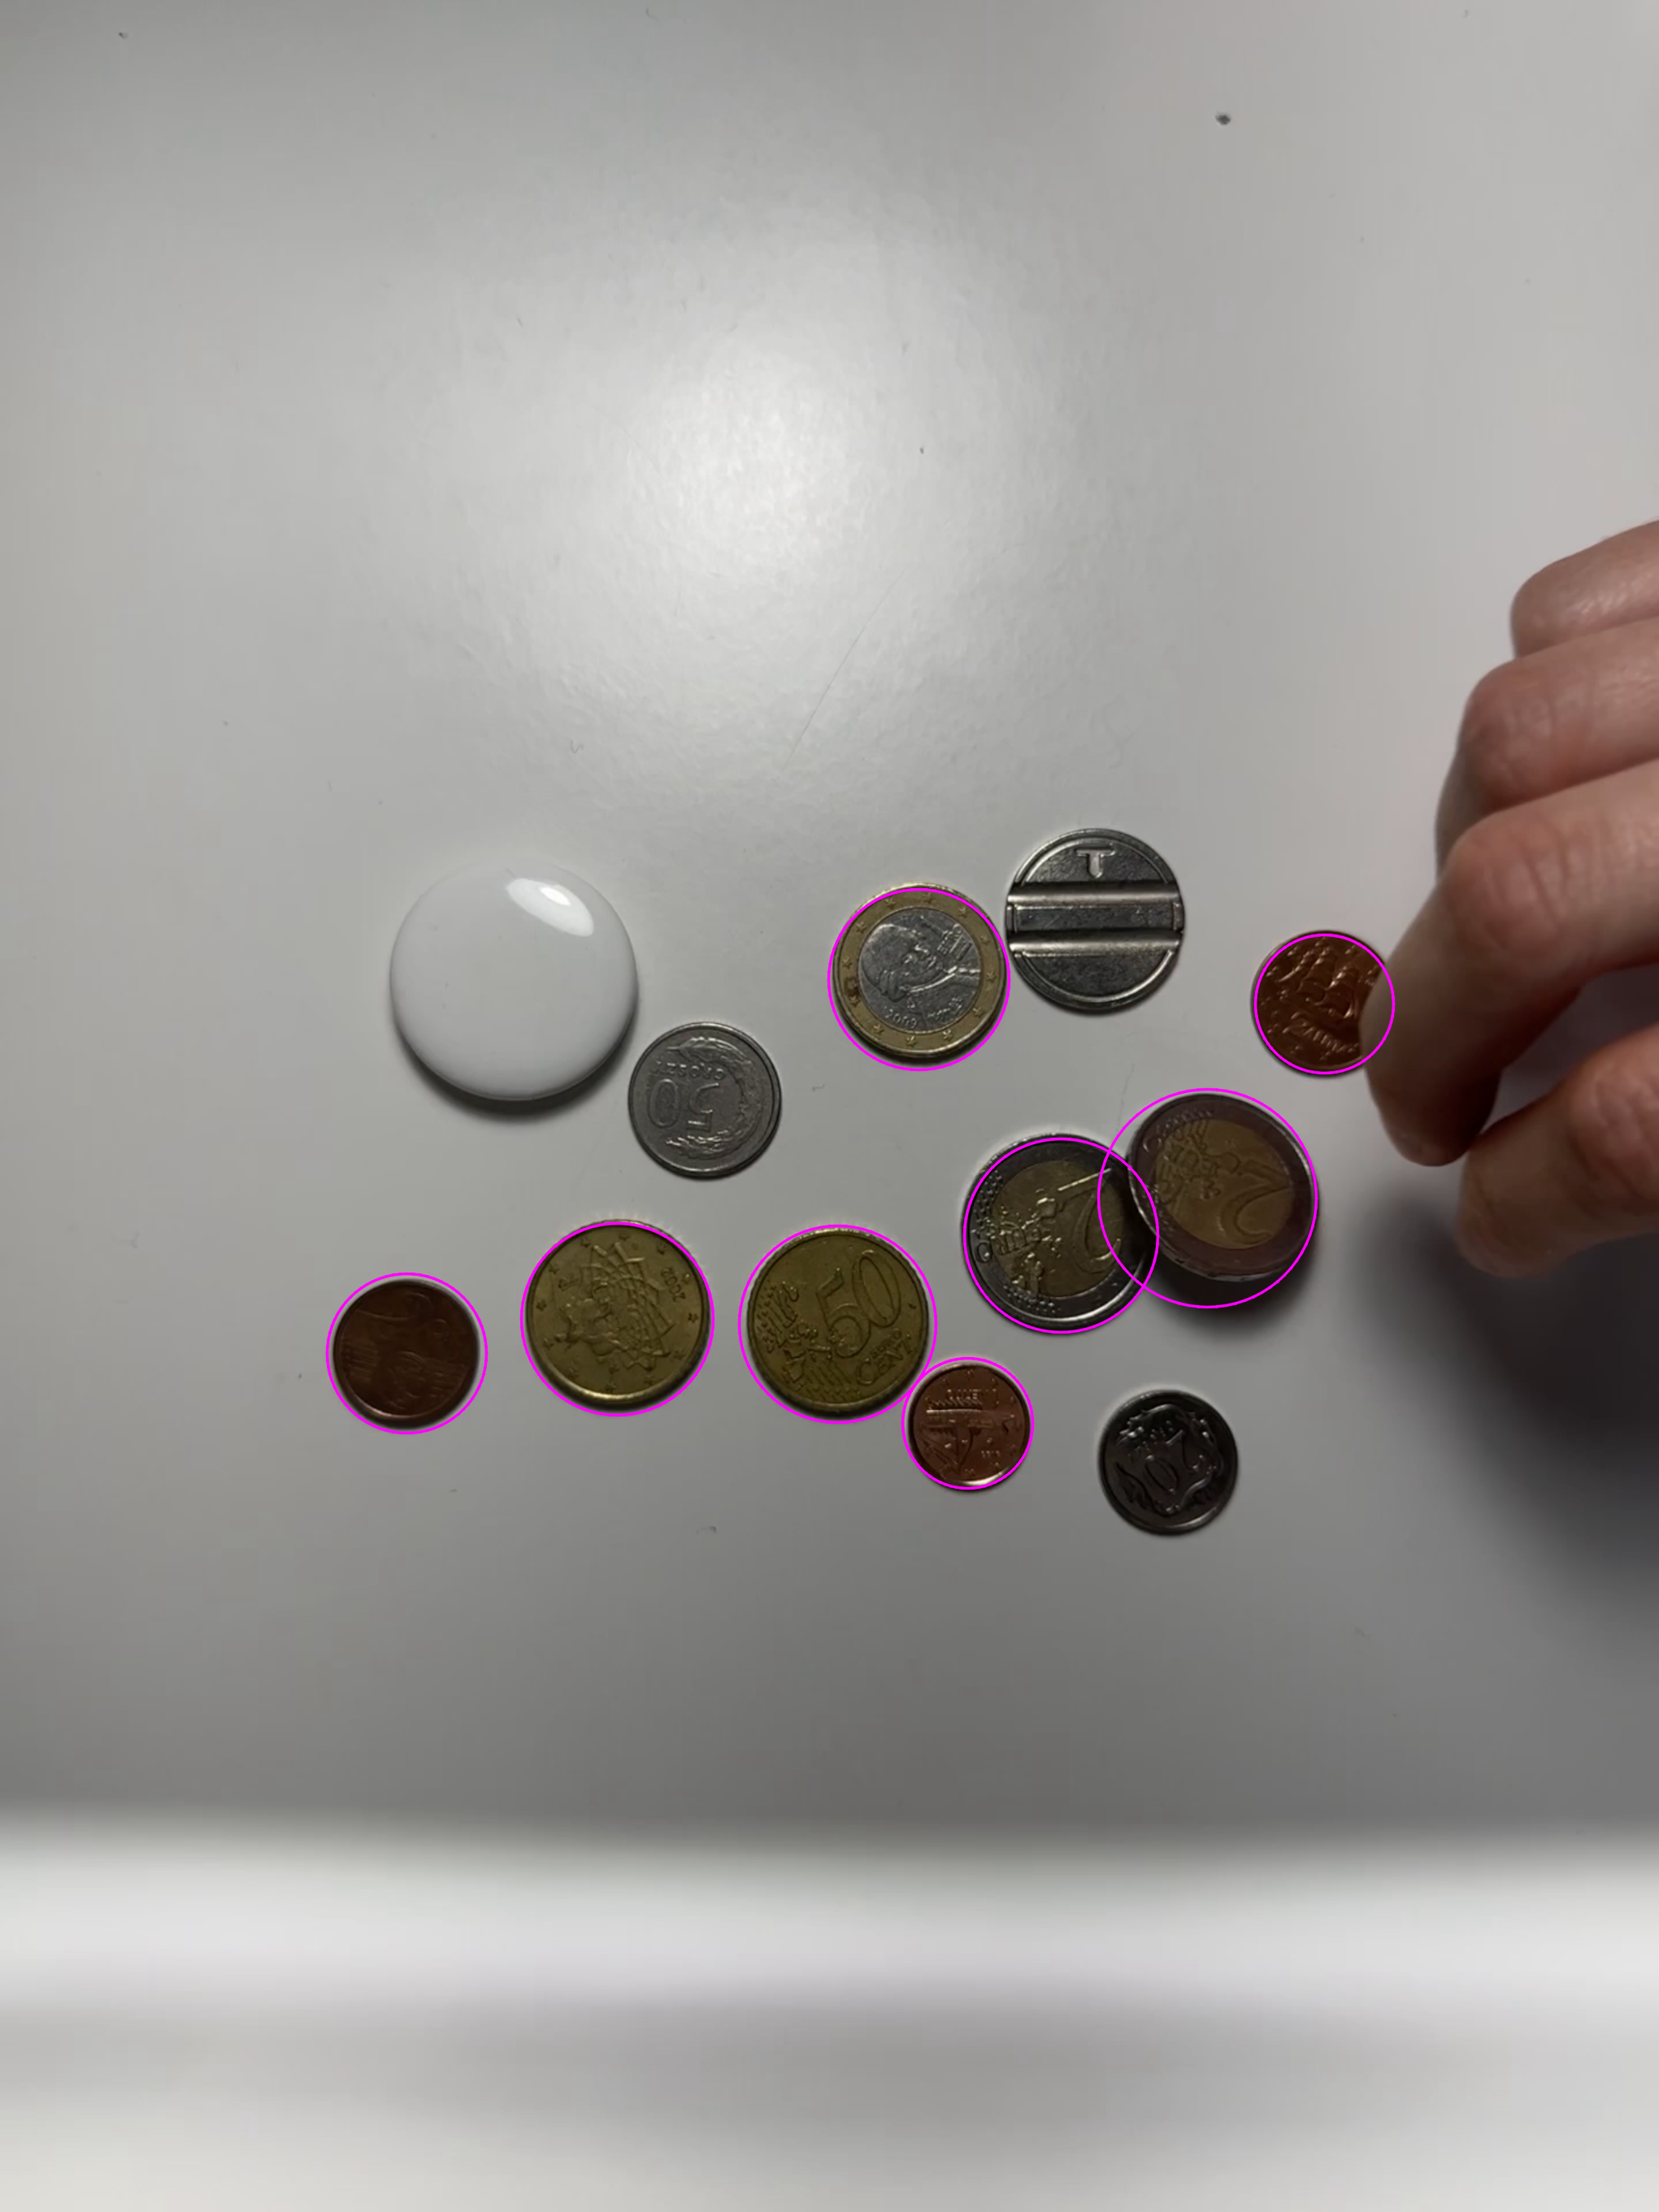
\includegraphics[width=0.35\textwidth]{Immagini/remaining_circles.png}
    }
    \caption{Filtering circles by color.}
    \label{Detection:fig:circle_detection_final}
\end{figure}